\section{NAX Analysis}
\subsection{Circulation Analysis}
Since the unissued portion of each issuance cycle is rolled into the following cycle and the total circulation supply is a fixed amount, the initial pre-issuance can be derived. If total issuance amount is  10 billion (\(10^{10}\)) NAX, then the scale of the 0th pre-release is as follows:
\begin{equation}
  \sum_{i,j} K_{i,j} = \sum_i C_0 \mu^i = \frac{C_0}{1-\mu}
\end{equation}
  Set the upper bound to 10 billion (\(10^{10}\)) and solve for \(C_0 = 10^{10}(1-\mu) = 1.0\times10^7\).

\subsection{Distribution ratio and pledge rate relationship}
The relationship between the ratio of issuance and the pledge rate, as shown in the figure \ref{func}. According to token demand, the value of the distribution ratio is between 0 and 1. For example, when the pledge rate is 30\%, the ratio of the issuance is 70% and when the pledge rate is 50%, the ratio of issuance is 90%. Where \(l=1.52\), \(m=-3.88\), \(l=3.36\).

\subsection{The relationship between weight and currency age}
In order to encourage users to participate in pledging early, and not to negatively effect the enthusiasm of new pledge users, we designed functions that will make early users relative to new users. The distribution weights vary depending on pledge age, however as the number of completed distribution cycles increase, the difference will be negilble. After 90 distribution cycles, the weight will stabilize, such as reaching $1$. 

In order to encourage new user participation in pledging, their weight does not start from 0.0 but instead from a initial foundation of $0.67$. Therefore, according to the above equation \ref{func}, we can review the corresponding coefficients, where \(a=0.005\), \(b=-0.3\), \(c=0.2\), the function is shown in \ref{weight}. 

It can be seen that the value of the effective weight is between 0.67 and 1; as pledge cycles increase, the weight increases until it reaches it's maximum weight of 1. After 30 pledge cycles (about 1 month), the effective weight is 0.8, after 60 pledge cycles (about 2 months), the effective weight is 0.9 and after 60 pledge cycles (about 2 months), the effective weight is 0.95.

\subsection{The impact of currency age on earnings}
In the case of the same number of pledges, the age of the coin generated by the initial pledge time will have an impact on the income. The magnitude of this effect is not very obvious. Below we give an example of the simulated effect as shown in the figure \ref{fig:compare}. Note: This figure is only for comparative reference and does not reflect actual revenue. In the case, the actual income is also related to the overall pledge quantity and address.
\begin{figure}[htbp]
  \centering
    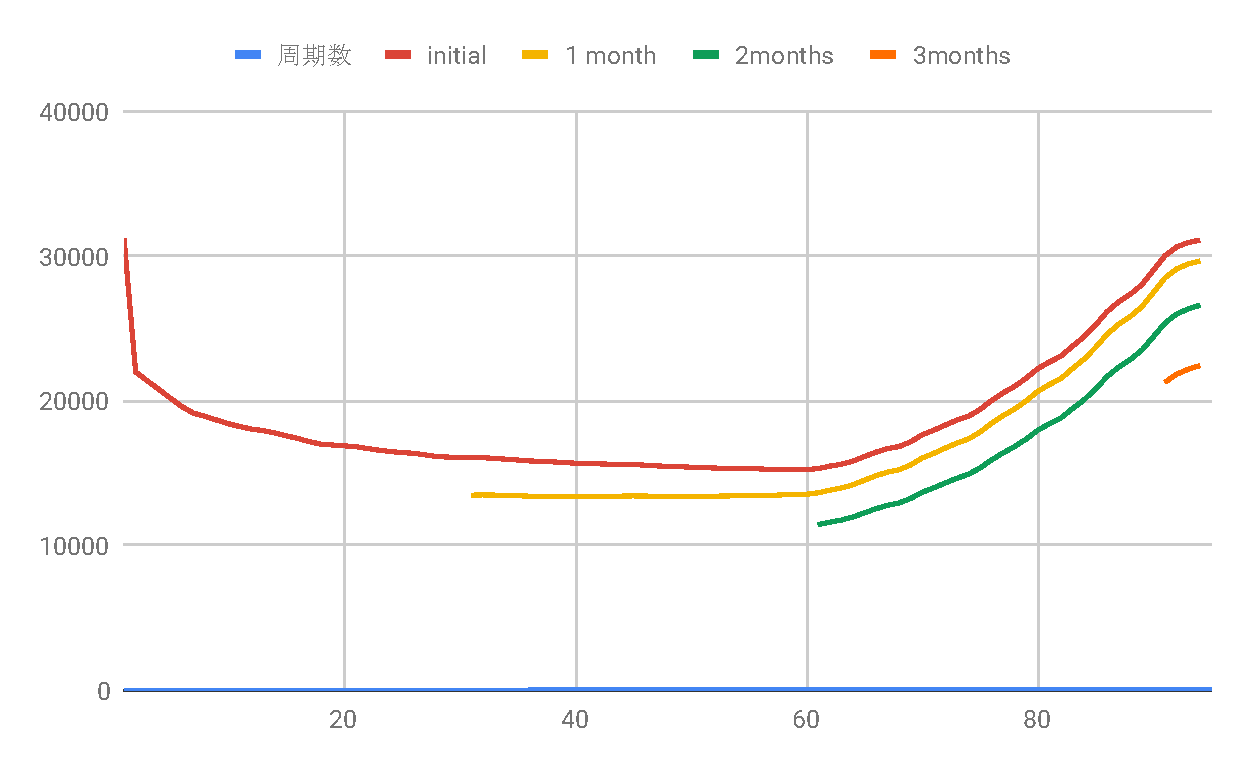
\includegraphics[width=0.6\textwidth]{../common/zh/compare.pdf}
    \caption{The effect of pledge start time on revenue\label{fig:compare}}
\end{figure}

\subsection{Initial issuance strategy}
Since our issuance method introduces a rollover distribution method, in order to make an early bird effect for those who initially pledge, we will issue the first issuance from $C_1$ and roll the full amount of $C_0$ to the first issuance cycle.
